\chapter{X-ray Detectors}
\label{chap:chapter2}

Since its birth in the 1960s \cite{giacconi2003}, X-ray astronomy has represented a powerful tool to study high-energy phenomena that involve celestial objects across the universe. The possibility to observe photons produced both by galactic and extragalactic sources, such as neutron stars, bynary sistems, supernova remnants or Active Galactic Nuclei (AGN), is made possible by the small probability of interaction with the low-density interstellar medium (ISM) and intergalactic medium (IGM) for energies above 0.1-1 keV. The crucial problem of X-ray astronomy arises when photons reach Earth's atmosphere, which is much denser than ISM and IGM, thus they are easily absorbed and can not reach the surface. Fig. \ref{fig:transparency} shows the altitude at which atmosphere becomes transparent as a function of the photon energy. For comparison, atmosphere's outer layers have a density of about $10^{17}$ atoms cm$^{-3}$, while for ISM the average on the galactic plane is $1$ atoms cm$^{-3}$ and for IGM is $10^{-6}$--$10^{-7}$ atoms cm$^{-3}$ \cite{longair2011}. The presence of the atmosphere makes it necessary to build space telescopes on board of satellites and send them into orbit around the Earth or the Sun. This is the reason why X-ray astronomy was born only after the progress of rocket science, when it became possible to launch the first detectors on sub-orbital flights, with which the first extrasolar sources were discovered, and then on satellites, which allowed to improve observations thanks to the increased available observation time and to fully dedicates missions. 

\begin{figure}[!b]
    \centering
    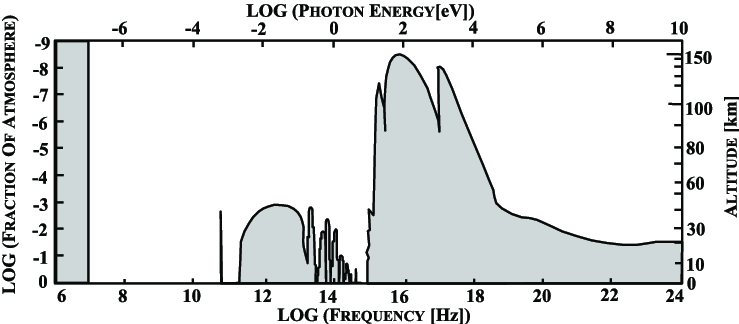
\includegraphics[width=0.7\linewidth]{figures/chapter2/transparency}
    \caption{Altitude above which the atmosphere becomes transparent for different frequecies of electromagnetic radiation. To observe soft X-rays (0.1--10 keV) it is necessary to reach altitudes above 80 km. The steep jump near 1 keV is due to photoelectric effect of nitrogen and oxygen. For hard X-rays (10--100 keV) and $\gamma$-rays ($>100$ keV) the minimum altitudes goes down to about 20--40 km. Image taken from \cite{transparency}.}
    \label{fig:transparency}
\end{figure}

This opportunity allowed to access a new perspective on the universe, which led to the discovery of new types of sources and to a better understanding of the physical processes that take place in astrophysical sources during high-energy events. An example is Scorpius X-1, the first detected extrasolar X-ray source and the most luminous persistent source of the X-ray sky. It has an X-ray luminosity about $10^3$ times larger than its optical counterpart, indicating that the emission processes are very different from those of the Sun, where the X-ray luminosity is about $10^{-6}$ times smaller than the visible light luminosity. Indeed, Scorpius X-1 is a Low Mass X-ray Binary system (LMXB) where a compact object, a neutron star in this case, accretes material from its companion and the emission is mainly due to the conversion of gravitational energy into thermal energy. Many other X-ray sources with various nature were discovered in the following years, such as active galactic nuclei, which are extragalactic sources where a supermassive black hole with a mass larger than $10^6$ M$_{\odot}$ accretes matter from the surrounding environment releasing enormous amounts of energy. All of these high-energy sources are united by the presence of extreme conditions, with gas heated to very high temperatures up to $10^{10}$ K or with high energy particles that interact with matter or magnetic fields producing high energy photons, both in the X and $\gamma$ regions of the electromagnetic spectrum. 

The limiting factor for the detection of X-rays is detector sensitivity. Indeed, the incoming fluxes from astrophysical sources are quite small. For reference, during active phases the Sun can reach a flux of $10^6$ ph cm$^{-2}$ s$^{-1}$ in the range 2-10 keV while Scorpius X-1 has a flux of about 30 ph cm$^{-2}$ s$^{-1}$ and 3C 273, the most luminous AGN, about 0.01 ph cm$^{-2}$ s$^{-1}$. The necessity to improve flux sensitivity, in order to discover fainter sources, has led the research and developement of X-ray detectors, which have evolved substantially across the years and have employed very different technologies.

\section{X-ray observables}

\fix{Qui potrei descrivere le 4 osservabili importanti nell'astrofisica X, che sono energia, imaging, timing e polarimetria. Per ogni osservabile descrivo quali importanti informazioni permette di ottenere (e.g. spettro -> informazioni su meccanimi di emissione, stato della materia, ...). Qualche foto carina di spettri, sorgenti e.g SN / AGN. Per il timing bisogna cercare un po di info, ma si può parlare brevemente delle pulsar in sistemi binari che permettono di effetuare verifiche di relatività generale ma anche di porre limiti alle EOS delle NS grazie alla misura della massa in sistemi binari. Per la polarimetria si può parlare dell'ambiente che circonda le sorgenti, in particolare campo magnetico, e quali info puo dare. Poi si può dare particolare enfasi all'importanza di avere tutte queste informazioni per una singola sorgente, e ancora di piu di effettuare questi studi nello stesso momento grazie a detector che sono capaci di fare piu cose. In particolare per studi di variabilità.}

The four observables that can be measured when a photon is detected are its energy, position, time of arrival and polarization, and each of them allows to understand different aspects of astrophysical sources.

The energy spectrum allows to understand the dominant emission processes of a source which can depend on its physical state, chemical composition and surrounding environment. A high-energy astrophysical source can have thermal or non-thermal emission processes, ...





\section{History of X-ray Astrophysics}
\label{section:history}

The first orbiting satellites to employ instrumentation to observe X-rays were part of the Orbital Solar Observatory (OSO) program, but they were mainly focused on the study of the Sun X-ray emission. Despite their main mission goals, they also performed some observations of galactic and extragalactic sources that allowed to confirm discoveries made by other missions with sub-orbital flights. However, without dedicated instrumentation it was not possible to carry on systematic studies of fainter sources. In this context, a major advancement was achieved with UHURU, the first orbital mission fully dedicated to X-ray observations of extrasolar sources, launched in 1970. Before UHURU, each sub-orbital flight was able to observe the sky for about five minutes, and during the entire 1960s only about an hour of observations was cumulatively gathered. With the launch of UHURU, observations were carried continuosly for over two years, collecting an amount of data many orders of magnitude larger than the entire previous decade. This satellite performed an all-sky survey, scanning a different region of the sky each day. The results allowed to discover more than 300 new sources \cite{4ucatalog}, localized with a precision of 1 arc min, enabling the identification of counterparts in other regions of the electromagnetic spectrum, such as visible and radio.

The heritage of UHURU was collected by the following missions that were part of the high-energy observatories program for X and $\gamma$ astrophysics, the three High Energy Astronomy Observatories (HEAO). One of the most important among them is HEAO-2, known as Einstein Observatory, launched in 1978. Einstein is, strictly speaking, the first true X-ray telescope, meaning that for the first time mirrors were used to focus X-rays onto a detector located in the focal point, marking the birth of imaging X-ray astronomy and paving the way to all the future detectors of this type. Until that moment, an X-ray observatory usually had a set of collimators to mechanically delimit the observed sky region. With different collimator geometries and with dedicated reconstruction algorithms it was possible to achieve a resolution of at most a few arc sec (about $7"$--$10"$ for HEAO-1 \cite{heao1a3}), but still it was not possible to produce images of extended sources. Moreover, a better spatial resolution in a collimator usually implies a decrease of the effective area, with the consequent drop of the signal-to-noise ratio. With Einstein Observatory these problems were solved using focusing optics. However, while for visible light a mirror surface reflects almost all the incoming photons, high-energy photons have a very high probability of penetrating the surface and thus not being reflected. The solution consists in using grazing incidence optics, relying on total reflection of light to have an increase of reflectivity. Indeed, this law holds for X-rays too, with the difference that the total reflection angle is usually below 1 degree and there is a quite strong dependence on the photon energy, making this method feasible only for low energy X-rays up to 10-20 keV. A possible optics geometry is the Wolter, named after its designer Hans Wolter, that consists in using two mirrors to focalize light at low incidence angles, usually one with parabolic section and one with hyperbolic or ellipsoid section. This layout allows to have a field of view large enough to be used in astrophysics and it is one of the reasons that makes it the most common layout between grazing incidence telescopes. The main issue of grazing incidence telescopes is the very small geometrical area due to the small inclination of the mirrors with respect to the optical axis. The natural solution to this problem is to use multiple nested concentrical mirrors to multiply the area, altough it introduces a series of technical and structural problematics that have been overcome in the years thanks to technological improvements. Einstein Observatory employed four nested mirrors with a diameter varying between 33 and 56 cm, a focal lenght of 3.4 m, a geometrical area of about 400 cm$^2$ and the capability of alternating four different detectors on the focal plane. For high resolution imaging, the effective area dropped down to 20 cm$^2$ at 0.25 keV and 5 cm$^2$ at 2 keV, with a spatial resolution of 2 arc sec \cite{heao2}. Other imaging and spectroscopy instruments on board were able to achieve an effective area between 100--200 cm$^2$. Results were remarkable and the first high-resolution images of X-ray sources were produced, allowing to study their morphology in a completely new electromagnetic band, even with a smaller effective area than HEAO-1. This was possible because, contrary to collimator observatories, the entire effective area was focused on a small region of the sky, reducing background signal and consequently increasing the signal-to-noise ratio and the instrumental sensitivity. Einstein Observatory produced a detailed catalogue with almost \num{5000} sources, even observing just a small fraction of the sky. For most of them the localization was accurate enough to identify their optical counterparts.

The successive step in the creation of a new and more populated all-sky catalogue was lead by ROSAT, launched in 1990. ROSAT had an overall design very similar to Einstein Observatory, but the optics layout consisted in larger and more efficient mirrors, that enabled to increase the effective area, and a different focal ratio, in order expand the field of view to faster scan the entire sky. Indeed, ROSAT had a field of view twice as large as Einstein and it also had a more uniform sensitivity across the field of view. In just 6 months, ROSAT was able to observe almost \num{150000} sources \cite{rosat}. During its nine years of operations, ROSAT also studied in detail many different sources, including emission from galactic stars and compact objects, spectral and morphological studies of supernova remnants. For the first time, it was also able to resolve the diffuse extragalactic emission into tens of thousands of AGN, giving a fundamental contribution to the development of the unified model and to variability studies. The limit of ROSAT was its narrow energy range, which was partially attributable to the mirrors geometry, that had a relatively big angle of inclination with respect to the focal axis to achieve a large field of view sacrifying sensitivity to higher energies, but was also due to the detectors employed to reveal X-rays. Indeed, the main imaging detectors types used until ROSAT were Position Sensitive Proportional Counters (PSPC) and Micro-Channel Plates (MCP). PSPC is a gas detector and it looses sensitivity at high energies because the gas becomes optically thin, with a consequent reduction of the quantum efficiency. For similar reasons, MCPs are unefficent at high energies, because X-rays easily penetrate the internal coating and glass. Furthermore, even though MCPs were the only way to achieve very good spatial resolutions, they are not capable to measure photon energy, requiring to alternate different instruments in the focal plane to study morphology and spectrum of a source.

\begin{figure}[htbp]
    \centering
    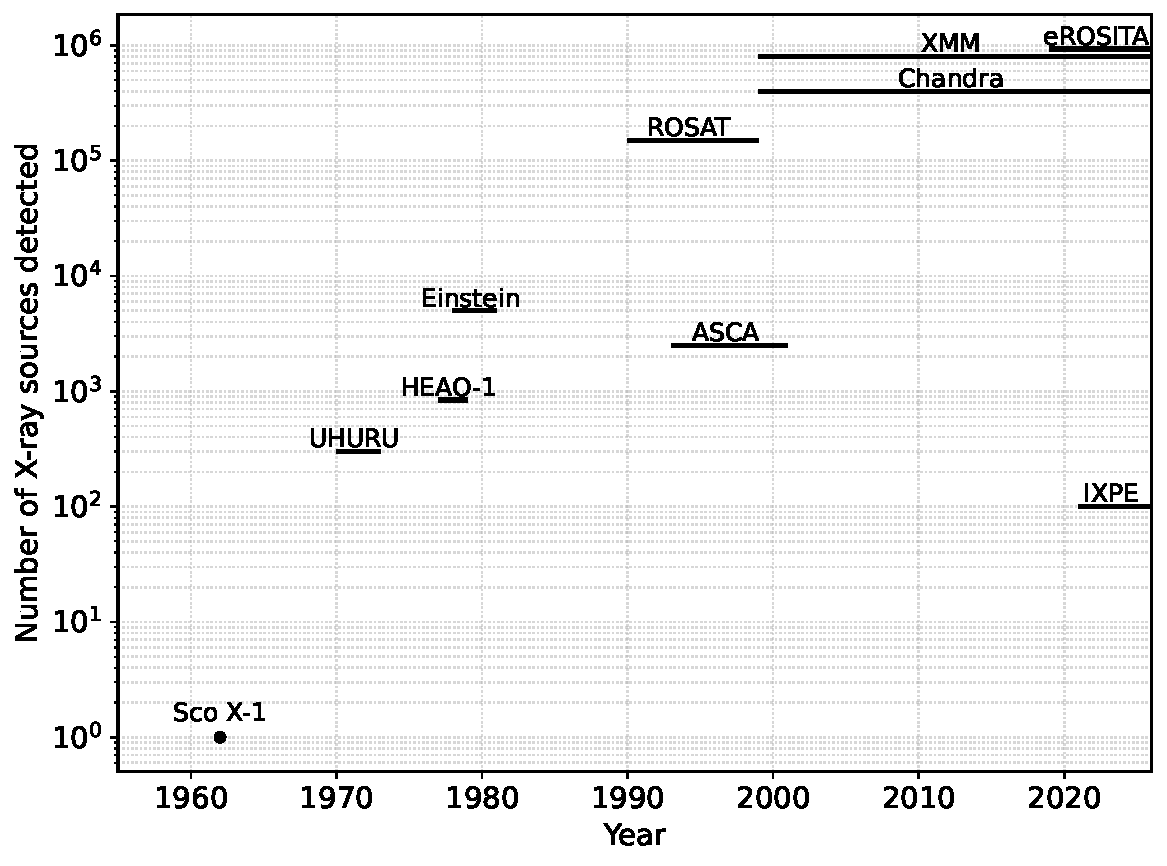
\includegraphics[width=0.7\linewidth]{figures/chapter2/xsources}
    \caption{Number of sources detected by the main X-ray observatories across the years. The horizontal lines represent mission lifetimes.}
    \label{fig:xsources}
\end{figure}


A new mission was launched in 1993 to overcome these limitations, Advanced Satellite for Cosmology and Astrophyisics (ASCA), with two revolutionary changes. The first was in the optics design, that for the first time in a space telescope were realized using a large number of nested concentric metal foils coated with a high-Z metal. ASCA had four telescopes, each with 120 nested gold-coated foils positioned with a very small angle with respect to the optical axis, increasing both the maximum observable energy up to 12 keV and the effective area, which reached 325 cm$^2$ at 1 keV for each telescope (when considering only the optics). The second innovation consisted in the use of CCDs as detectors in the focal plane, the first time for an X-ray telescope. With the use of CCDs in photon counting mode it became possible to perform high resolution imaging and spectroscopy of the source at the same time, even at high energies.

The first generation of X-ray CCDs suffered from various problems, such as low quantum efficiency both at low and high energies, with the latter caused by a small depletion region, and electronical issues were responsible for spectral resolution deterioration. These problems were solved by the following generation of X-ray observatories, with Chandra and XMM-Newton, both launched in 1999 and currently operational. These two missions pushed to the limit the technological advancement of CCDs. XMM-Newton is the first X-ray observatory to employ a high thickness and fully depleted CCD \cite{xmm_pn}, ensurin high quantum efficiency in the entire operational energy range, which reaches 15 keV. On the other hand, Chandra's CCDs were optimized for low energy X-ray photons and spatial resolution, improving the readout electronics to decrease noise and also reducing the pixel size, in order to take full advantage of the 10 meters long focal length and achieve a spatial resolution of $0.5$ arc sec \cite{chandra}. Fig. \ref{fig:sensitivity} shows a measure of the sensitivity of some of the cited observatories by estimating the observed surface source density above a certain flux threshold.

\begin{figure}[htbp]
    \centering
    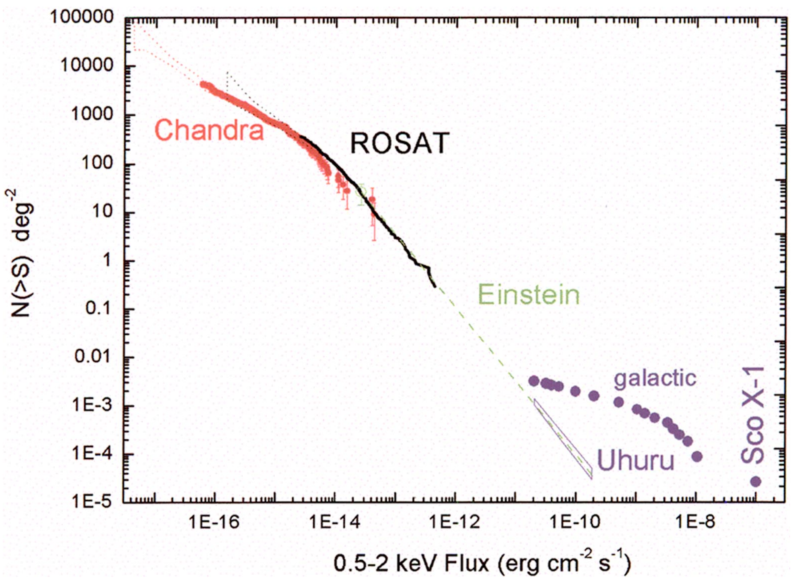
\includegraphics[width=0.7\linewidth]{figures/chapter2/sensitivity}
    \caption{Sensitivity of some X-ray observatories across the years, represented as number of sources with flux above a threshold $S$ observed in a square degree of sky as a function of the flux $S$ between 0.5 and 2 keV. The lower limit for each observatory is an indicator of the minimum observable flux. The slope of the curves is an indicator of how the sources are distributed across the universe. In case of UHURU the slope is different because the majority of sources are galactic, thus they have a different spatial distribution. Image taken from \cite{giacconi2003}.}
    \label{fig:sensitivity}
\end{figure}

Beyond imaging and spectroscopy, polarization of X-ray emission from a source can be studied to infer important properties about its surrounding environment, such as magnetic fields, and the physical mechanisms at play \cite{xray_polarimetry}. The first successful X-ray polarimetry mission took place in 1971 and was carried out with sub-orbital rockets using a crystal Bragg polarimeter, resulting in the first measure of the polarization level of the Crab Nebula. This type of detector consists in a crystal of a specific material, which defines a narrow energy sensitivity band, mounted at an angle of 45 degrees with respect to the incident flux. If a photon has the electric field vector parallel to the crystal surface it is reflected, otherwise it penetrates the crystal and is absorbed. By counting the photons that are reflected as a function of the azimuthal angle while the detector is spinning around the axis that points towards the source, it is possible to measure the level of polarization. For many years this method represented the only feasible way to measure X-ray polarization, but there were many physical and technical problems associated to it. First of all, the energy range is very narrow, thus the observed rate is small and the consequence is that even for bright sources the observation time required to detect polarization is very long. The second big problem is technical, because it is difficult to make the detector spin pointing exactly towards the source, with the possibility of introducing systematics errors that could false the polarization. For these reasons a mission completely oriented to X-ray polarimetry was never realized until a new technique to measure was developed. This new method consists in using the dependence of the direction of motion of primary photoelectrons released in photoelectric absorption on the polarization. Tracking the motion of electrons after absorption allows to reconstruct the initial angle. This is the operational basis of Imaging X-ray Polarimetry Explorer (IXPE), launched in 2021, where Gas Pixel Detectors (GPD) are employed. IXPE allows to reach high sensitivity with observing times at least two orders of magnitude lower than old missions. Another important aspect of IXPE is its ability to provide not only polarization data of the observed source, but also imaging, spectral and timing data at the same time. More details about IXPE and its detectors will be given in Chap. \ref{chap:chapter3}.

\begin{table}[htbp]
\centering
\small
\begin{tabularx}{\textwidth}{l l X c c}
Mission & Lifetime & Main instruments & Energy [keV] & Eff. Area [cm$^2$] \\
\toprule
UHURU 	 & 1970--1973   & Proportional counters & 2--20 & 840 \\
\addlinespace
Einstein & 1978--1981   & PSPC & 0.4--4.0 & 100 \\
         &              & Microchannel plates & 0.15--3.0 & 5--20 \\
\addlinespace
ROSAT	 & 1990--1999   & PSPC & 0.1--2.5 	& 240 \\
         &              & Microchannel plates & 0.1--2.5 & 80 \\
\addlinespace
ASCA 	 & 1993--2001   & CCD	& 0.4--12 & 105 \\
		 &				& Gas scintillation PC & 0.8--12 & 50 \\
\addlinespace
Chandra	 & 1999-- 		& CCD & 0.2--10 & 340 \\
		 & 				& Microchannel plates & 0.1--10 & 225 \\
\addlinespace
XMM 		 & 1999-- 		& CCD MOS & 0.1--15 & 922 \\
		 & 				& CCD PN  & 0.1--15 & 1227 \\
\addlinespace
IXPE		 & 2021-- 		& Gas pixel detector	  & 2--8	  & 167 	  \\

\bottomrule
\end{tabularx}
\caption{Some of the X-ray missions representing the technological evolution of X-ray detectors and telescopes, from collimators to grazing incidence optics and from gas proportional counters to solid state pixel detectors for imaging and spectroscopy and Gas Pixel Detectors for polarimetry.}
\label{tab:missions}
\end{table}


\section{Light-matter interaction mechanisms}
There are three main mechanisms with which high energy photons can interact with matter, which are photoelectric effect, Compton scattering and electron-positron pair production. These processes are at the basis of photon detection and are commonly employed in the construction of high-energy photon detectors \cite{longair1992, leo1994}.

\fix{Forse bisogna inserire qualcosa di generico sulla lunghezza di assorbimento, ma non nel fotoelettrico.}

\subsection{Photoelectric effect}
When a photon has an energy $E_{\gamma} \ll m_e c^2$ the main interaction process is photoelectric effect, which consists in a photon that is absorbed by an atom with the consequent ejection of a free electron

\begin{equation}
\gamma + (A, Z) \rightarrow e^- + (A, Z)^+.
\end{equation}

A photon with energy $E_{\gamma}$ can be absorbed and cause the ejection of an electron only if $E_{\gamma} \geq E_B$, where $E_B$ is the binding energy of the involved electron. The electron is expelled with a kinetic energy equal to $E_{\gamma} - E_B$. The atomic energy level structure can be observed from the appearance of jumps in the photoelectric cross section, which are referred to as absorption edges. Atomic electrons are arranged in shells, with increasing binding energy from the outermost to the innermost one. When a photon has enough energy to interact with a more internal shell, the cross section rapidly increases. In heavy elements with high atomic number $Z$, the large binding energy difference between orbitals inside the same shell is responsible for the apperance of further small edges. The photoelectric cross section usually has a strong dependence on the photon energy and on $Z$, and for the K-shell, corresponding to the innermost $1s$ spherical shell, it scales as

\begin{equation}
\sigma_{K} \propto E_{\gamma}^{-3.5}Z^5.
\end{equation}

Outer shells have a strong dependence on energy and atomic number as well, but it gradually decreases going outwards. Fig. \ref{fig:photo_cross_section} shows photoelectric cross section dependence on energy for silicon ($Z = 14$) and for the compound material cadmium-telluride CdTe, a crystal made by cadmium and tellurium ($Z_{Cd} = 48$, $Z_{Te} = 52$). For both materials is possibe to observe the increases in the cross section corresponding to the K-edge, while for CdTe there is also the L-edge. Because of the large difference between the atomic numbers, CdTe has a cross section almost $10^3$ times larger than silicon for energies above the K-edge at about 30 keV.

Once the photoelectron has been ejected, the atom is in an excited state and there are two major mechansisms with which it can return to the ground state. Generally, an electron from an outer shell fills the vacancy caused by the photoelectric effect and the difference is in the later de-excitation process. The first process consists in the emission of an Auger electron, which happens when the electron that filled the vacancy transfers energy to an electron in the outer shells, causing the ejection of the latter with a kinetic energy that corresponds to almost the entire de-excitation energy. Furthermore, the emission direction is isotropic. The second process is X-ray fluorescence emission, which happens when the energy is released by emitting a photon with energy corresponding to the binding energy difference between the vacancy and the outer electron levels. After this processes, the atom is then left with one or two vacancies in the outer shells that, depending on the state of the material, can be filled by recombination, with consequent emission of low energy photons, or by non-radiative thermal dissipation. The probability of emitting fluorescence radiation instead of an Auger electron, called fluorescence yield, depends on the atomic number and on the shell. Fluorescence yield generally increases with $Z$ and for inner shells, as shown in Fig. \ref{fig:fluorescence_yield}, and it becomes dominant for atoms from $Z \approx 30$.

\begin{figure}[h]
    \centering
    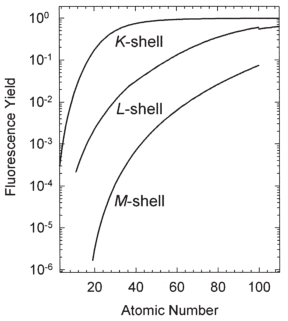
\includegraphics[width=0.45\linewidth]{figures/chapter2/fluorescence_yield}
    \caption{Fluorescence yield for elements $3 \leq Z \leq 110$ for K, L and M shells. Values showed for L and M shells represent the average between subshells. Plot taken from \cite{xraydatabooklet2009}.}
    \label{fig:fluorescence_yield}
\end{figure}

Another important property of photoelectric effect is its dependence on the photon polarization. When considering absorption by spherical shells, the differential cross section is \cite{muleri2008}

\begin{equation}
\frac{d \sigma}{d \Omega} \propto \frac{\sin^2 \theta \cos^2 \phi}{(1 + \beta \cos \theta)^4},
\end{equation}
where $\phi$ is the angle between the polarization vector and the direction of emission of the photoelectron, and $\theta$ is the polar angle, which measures the angle between the incidence direction of the photon and that of emission of the photoelectron. This dependence can be exploited to measure the degree of polarization of a source, which can be inferred by tracking photoelectrons and studying counts distribution as a function of $\phi$, which is equal to

\begin{equation}
N(\phi) = A + B \cos^2(\phi - \phi_0),
\end{equation}
where $A$ and $B$ are the parameteres that describe the degree of polarization. \fix{add other info?}

\subsection{Compton scattering}

\begin{figure}[t]
    \centering
    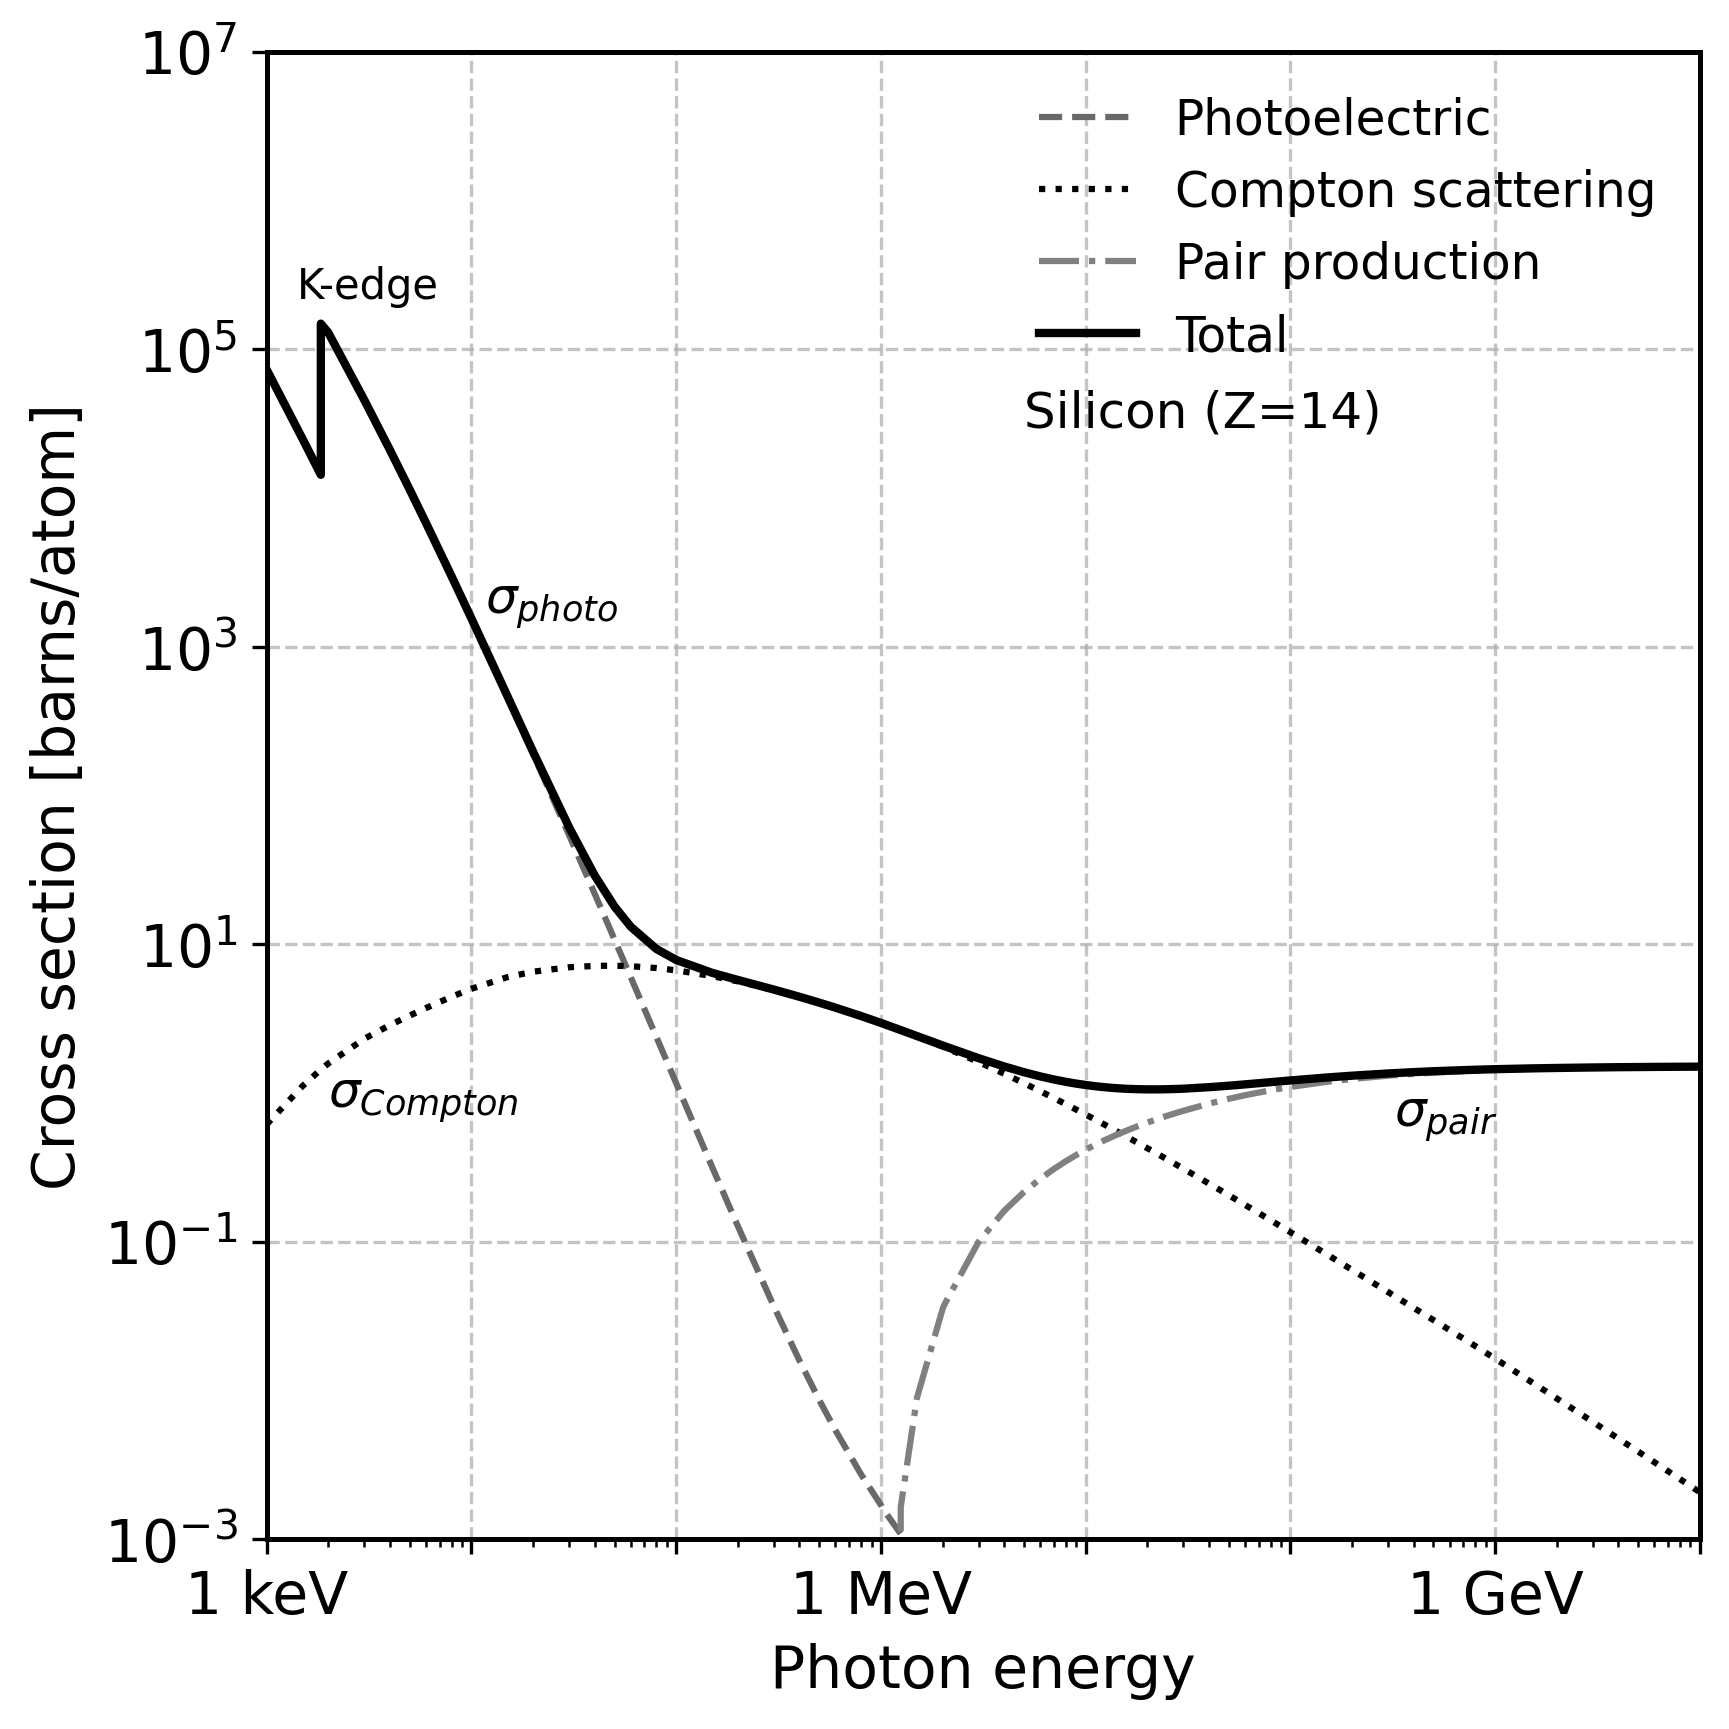
\includegraphics[width=0.49\linewidth]{figures/chapter2/si_cross_section}
    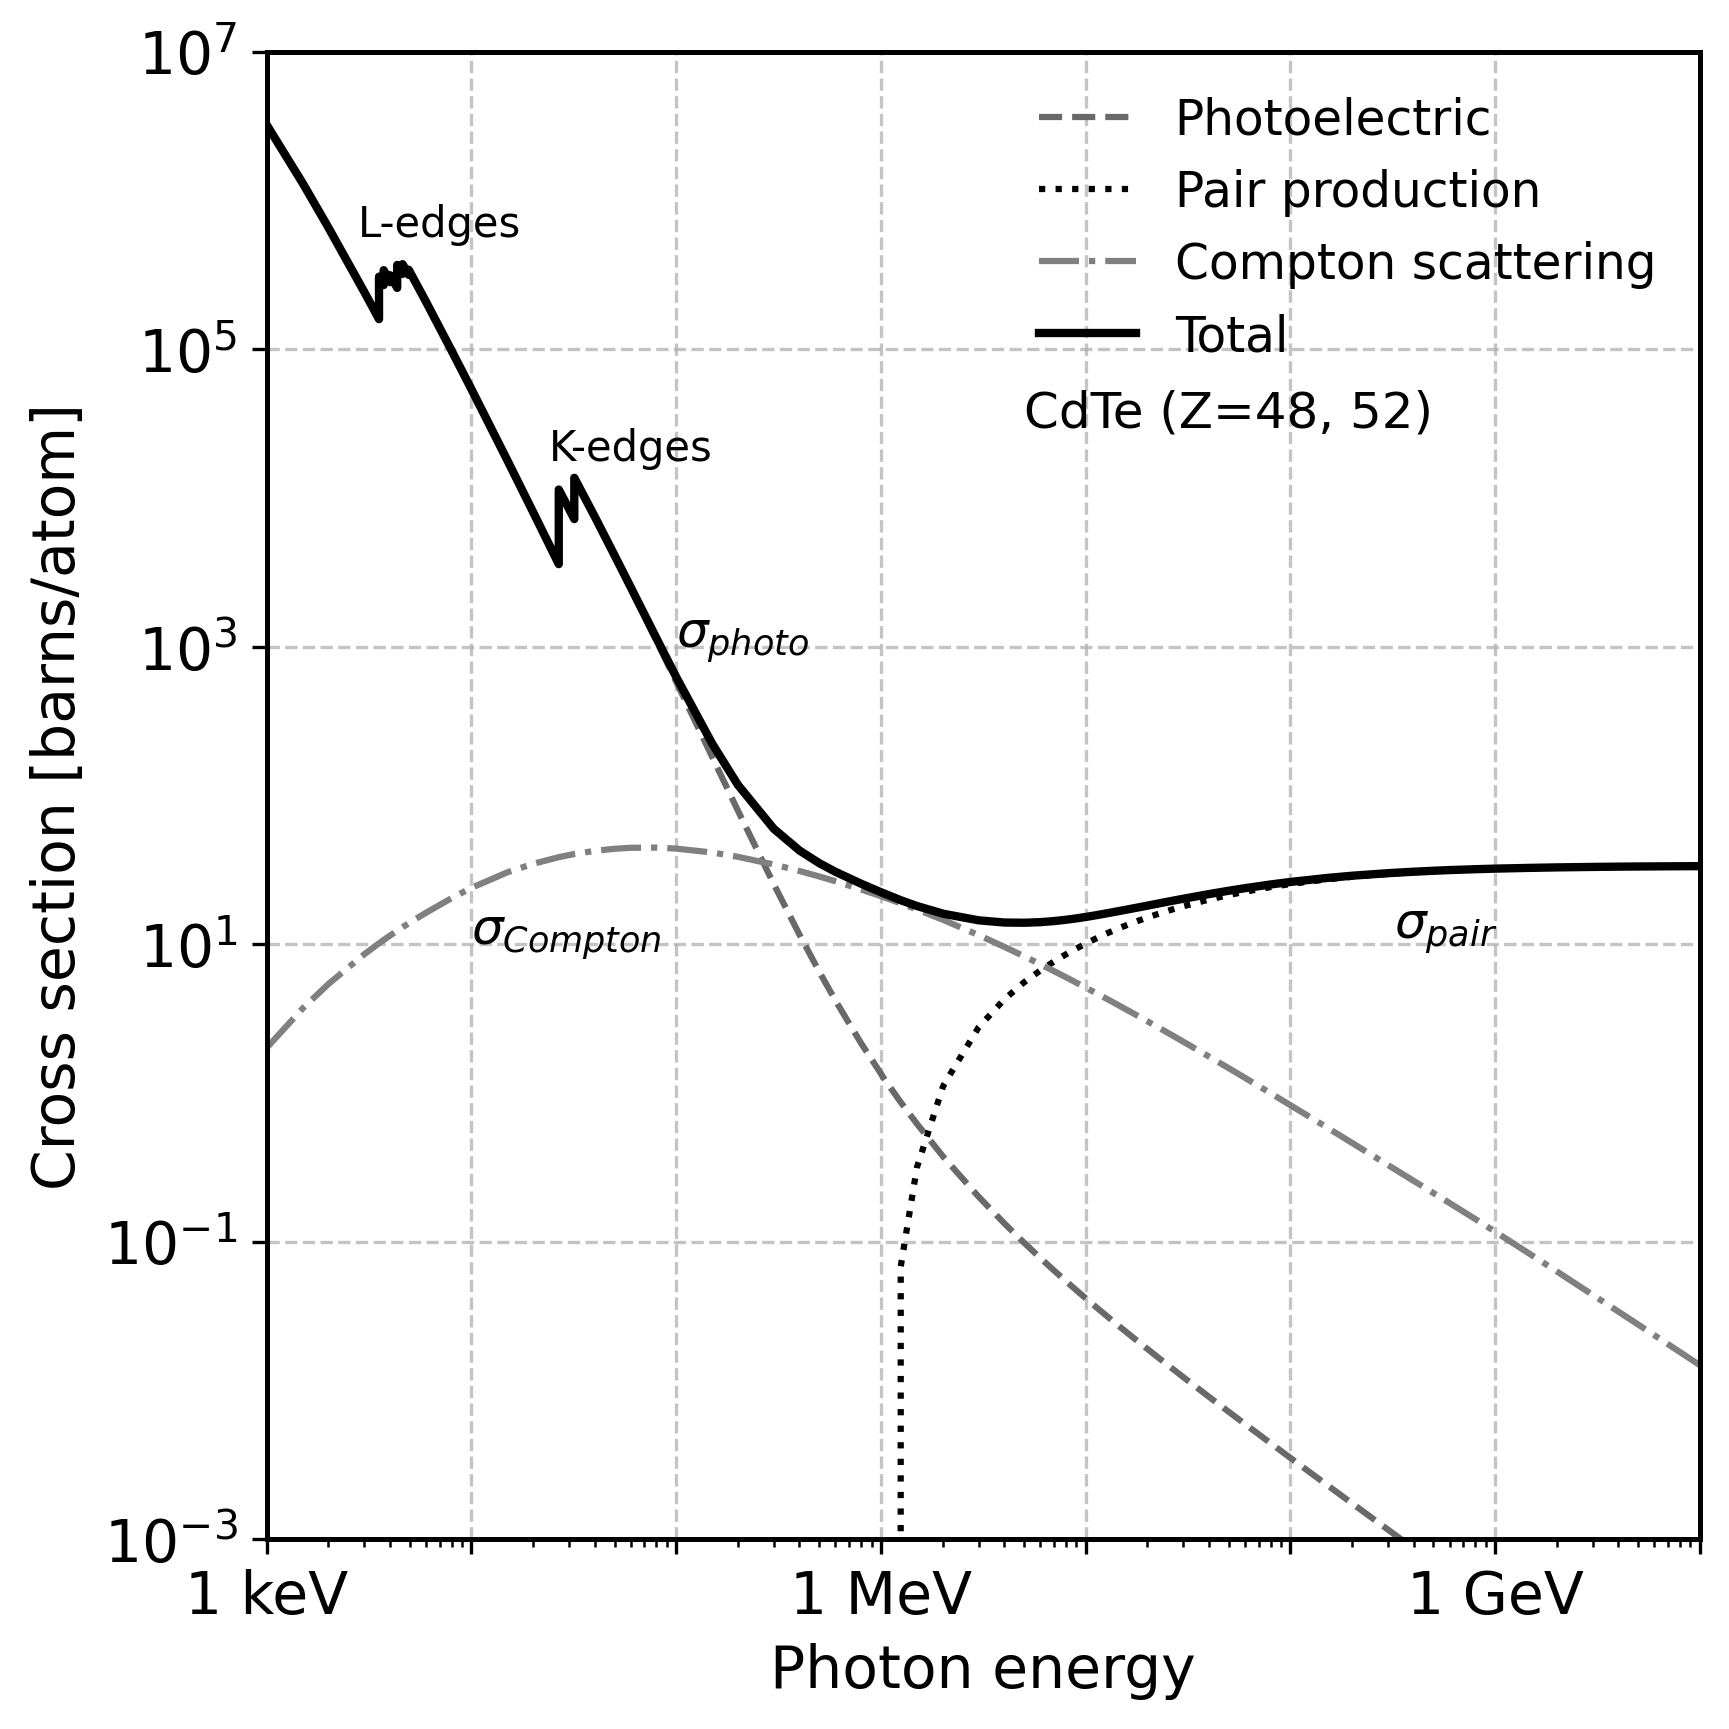
\includegraphics[width=0.49\linewidth]{figures/chapter2/cdte_cross_section}
    \caption{Photoelectric effect, Compton scattering, pair production and total cross sections for silicon (left panel) and cadmium-telluride (right panel). Photoelectric effect is the dominant process for energies up to 50--100 keV. K-edge is visible for silicon and CdTe at 1.8 keV and 27--31 keV, respectevely. L-edges are also visible for CdTe, at an energy of about 4 keV. Compton scattering is dominant from these energies up to 10 MeV, where pair production becomes the prevailing process. Data are gathered from \cite{nist_xcom}.}
    \label{fig:photo_cross_section}
\end{figure}

Compton scattering is the dominant interaction mechanism at higher energies. This process consists in the interaction between a photon and a free electron, with the photon that transfers part of its energy to the electron. It can be represented as

\begin{equation}
\gamma + e^- \rightarrow \gamma + e^- .
\end{equation}

Given the high energy at which the Compton effect becomes relevant, which is much larger than the energy of the K-edge, the assumption that an atomic electron is free and at rest is a good approximation.

In the frame where the electron is at rest, the photon energy after the interaction is

\begin{equation}
E_{\gamma}' = \frac{E_{\gamma}}{1 + \frac{E_{\gamma}}{m_e c^2}(1 - \cos \theta)},
\end{equation}
where $E_{\gamma}$ is the initial energy and $\theta$ is the angle between the photon initial and final directions. The differential cross section for polarized photons is given by the Klein-Nishina formula

\begin{equation}
\frac{d \sigma_{\textrm{C}}}{d \Omega} = \frac{r_e^2}{2} \left( \frac{E_{\gamma}'}{E_{\gamma}} \right)^2 \left( \frac{E_{\gamma}'}{E} + \frac{E_{\gamma}}{E_{\gamma}'} - 2 \sin^2 \theta \cos^2 \phi \right),
\label{eq:compton}
\end{equation}
where $r_e$ is the classical electron radius, $\phi$ is the azimuthal angle measured with respect to the polarization vector and $\theta$ is polar angle. When considering an atom with atomic number $Z$, the total Compton cross section scales as $\sigma_{\textrm{tot}} \propto Z \sigma_{\textrm{C}} $, showing a much weaker dependence on $Z$ compared to photoelectric effect. Fig. \ref{fig:photo_cross_section} shows the total Compton cross sections for silicon and CdTe, compared to other interaction mechanisms cross sections. The interval where the Compton effect is dominant becomes narrower for large atomic numbers. 

As for photoelectric polarimetry, Eq. \ref{eq:compton} is useful to measure polarization for higher energy photons. Indeed, Compton polarimeters are commonly used to study polarimetry in the hard X-ray and soft $\gamma$-ray bands, in the energy range from a few tens of keV up to a few MeV. 

\subsection{Pair production}
For energies above 10 MeV, in the $\gamma$-ray band, the dominant process becomes electron-positron pair production in the nuclear field, represented by

\begin{equation}
\gamma + X \rightarrow X + e^+ + e^- .
\end{equation}

This process can cinematically take place only if the photon has an energy above threshold $E_{\gamma} > 2 m_e c^2$. For an atom with atomic number $Z$, the total cross section scales as 

\begin{equation}
\sigma_{\textrm{pair}} \propto r_e^2 Z^2.
\end{equation}

At low energies, the cross section increases logarithmically with the photon energy, while at high energies it becomes constant, as shown in Fig. \ref{fig:photo_cross_section}, both for silicon and CdTe.

In high energy astrophysics, this process is exploited in pair production telescopes for $\gamma$-rays, where the produced electron and positron are tracked to determine the incoming photon direction and their energy is measured with an electromagnetic calorimeter to gauge the initial photon energy.

\section{Working principles of X-ray detectors}
As said above, photoelectric effect is the dominant interaction process in the X-ray energy band. For this reason, the following discussion is focused on photon detectors that employ this effect to convert an incoming photon into an interpretable signal which allows to measure one or multiple properties among energy, position, time of arrival and polarization.

Various detectors have been devoleped across the years and used on board of X-ray missions, each of them suitable for measuring one or multiple photon properties in a specific energy interval. The technology empolyed in the construction of these detectors can vary a lot but all of them share the same working principles to convert photons in a readable signal. First, photons interact with the active material through photoelectric effect and are absorbed, producing a photoelectron. This electron can have a lot of kinetic energy and it is transfered to the active material by collisions. The amount of energy lost by collisions is described by the Bethe-Bloch formula

\begin{equation}
- \frac{dE}{dx} = 2 \pi N_A r_e^2 m_e c^2 \rho \frac{Z}{A} \frac{1}{\beta^2} \left[ \ln \left( \frac{2 m_e \gamma^2 v^2 W_{\textrm{max}}}{I} \right) - 2\beta^2 \right].
\end{equation}

In ionization detectors, the energy transfered by the photoelectron ionizes atoms and molecules generating a large number of charge carriers, which in turn induce a current during their motion. Alternatively, in scintillators molecules are excited by the photoelectron and the signal is represented by the luminous emission produced by the de-excitation, which then is collected, converted and amplified to generate an readable electric signal.

The focus of this section is to briefly discuss which are the main ionization X-ray detectors and how they work. These detectors can be divided in two macro-groups, gas and solid state detectors, and are more suitable for soft X-rays detection, but can be adapted to detect hard X-rays as well by varying materials and working points. Hard X and soft $\gamma$ rays detection was dominated by scintillation detectors in the past, but in the last two decades solid state ionization detectors made with high-$Z$ materials have increasingly replaced them. 

\subsection{Gas ionization detectors}
The first X-rays detectors to be launched in space were gas detectors, thanks to decades of experience and development in ground-based experiments and to their low weight, which is essential to launch a satellite in orbit. A gas detector generally consists in a closed chamber filled with pressurized gas. A photon interacts with the gas and the photoelectron ionize it, generating a certain number of free electrons and ions. The number of electron-ion pairs produced after the interaction with a photon is stochastic and depends on the energy and the gas properties. The mean number of electron-ion pairs can be calculated as

\begin{equation}
N = \frac{E}{w},
\end{equation}
where $w$ is a quantity specific to a material and represents the mean energy necessary to create a pair. For gases this value ranges between 20 and 40 eV. As a first approximation, the number of pairs is distributed according to a Poisson distribution, thus the variance is given by the mean number of pairs produced. However, if all the incoming energy is absorbed by the gas, as is the case of X-ray photons, an additional constraint is added, because the number of pairs that are produced and the energy required to generate them is fixed by the photon energy. This means that pair production events are not independent, thus the Poisson distribution approximation is no longer valid. Under these hypotheses the variance is

\begin{equation}
\sigma^2 = F N,
\label{eq:fano}
\end{equation}
where $F$ is called Fano factor. Tab. \ref{tab:w_fano} shows the mean ionization energy and Fano factor for some common materials used for ionization detectors. For most of materials, including gases and semiconductors, $F < 1$. Therefore, when the amount of deposited energy is fixed, the variance is smaller. The energy resolution of the detector can be estimated with the assumption that for a large number of events the number of pairs is distributed according to a Gaussian distribution with the variance obtained from \ref{eq:fano}. The relative energy resolution at the energy $E$ is defined as
 
\begin{equation}
\frac{\Delta E}{E} = \frac{\operatorname{FWHM}}{E} = 2.35 \frac{\sqrt{F N}}{N} = 2.35 \sqrt{\frac{F w}{E}}.
\end{equation} 

The final energy resolution is the sum of more contributes, as other sources of uncertainties must be taken into account, such as electronic noise and all the other possible instrumental noise sources.

\begin{table}[htbp]
\centering
\small
\begin{tabularx}{\textwidth}{X c c}
Material & Mean energy for pair creation [eV] & Fano factor \\
\toprule
Argon &  & \\
Xenon &  & \\
Silicon & & \\
Cadmium-telluride &  & \\
\bottomrule
\end{tabularx}
\caption{Mean energy for pair creation and Fano factor values for various gases and semiconductors. \fix{fillare la tabella, che altri materiali posso mettere?}}
\label{tab:w_fano}
\end{table}

In gas, only a few hundreds electron-ion pairs are produced after the interaction of a photon with an energy of a few keV. Furthermore, pairs are produced in a small and localized region, and without an external field that separate them they would recombine before it would be possible to detect the signal. These are the reason why gas-ionization detectors usually have a drift region and a multiplication region, both employing an external electric field to separate or accelerate charges.

In the drift region, an electric field of the order of 1 kV/cm is responsible for the separation of electron-ion pairs to avoid recombination. Charges are accelerated under the work of the electric field, which is generated applying a potential difference between electrodes. The geometry of electrodes can significantly vary between different detectors, with some examples represented by the axial geometry of cylindrical proportional counters or planar geometry. Inside the drift region charges are subjected to diffusion processes due to collisions and thermal agitation. If no external field is present along an axis, charges are distributed according to a Gaussian distribution, with standard deviation equal to

\begin{equation}
\sigma = \sqrt{2D t_d},
\end{equation}
where $D$ is the diffusion coefficient, which depends on the material and on the working conditions (such as pressure or temperature), and $t_d$ is the drift time, which depends on the charge carriers mass and on the applied electric field. This holds along each axis where an external field is not applied.

The multiplication region is where charges are multiplied and it is achieved by accelerating charges with a strong electric field, with typical peak values of the order of 100 kV/cm. The kinetic energy is used by the charges to start an avalanche by further ionizing the gas, producing new electron-ion pairs that are accelerated by the electric field and in turn continue to ionize the gas. The induced current produced by the charges generates an amplified signal that exceeds electronic noise and can be read and processed. Depending on the voltage applied to the electrodes and the resulting intensity of the electric field, charge multiplication has different working regimes. At low voltages no multiplication process takes place and pair recombination is the dominant process. At higher voltages recombination is not favored, and in a certain interval multiplication occurs and the number of final electron-ion pairs is proportional to the number of primary ionization pairs. The ratio between the initial and final number of pairs represents the gain of the detector. This property is essential for spectroscopy, as it is possible to reconstruct the photon energy. In this voltage interval, which is called proportional counting region, gain grows exponentially with the voltage

\begin{equation}
G = e^{a V}.
\end{equation}
When the voltage becomes too high, the response becomes non-linear and even few ionization events produces a large pulse. This regime is called Geiger-Muller region. Detectors working in this regime are able to detect radiation but can not 

Charge multiplication can be obtained with various designs, going from electrodes disposed as in a cylindrical proportional counter to more complex and miniaturized designs, such as in micro-strip gas chambers or two-dimensional patterns like Gas Electron Multipliers (GEM).

The detector that flew on board of the first dedicated orbital mission, UHURU, consisted in a set of proportional counters. The external part of a proportional counter is usually a thick metallic case, which serves as the cathode, with thin windows of beryllium or plastic material that allow to suppress photons with energies below a few keV. The anode is a thin metallic wire positioned in the middle and running along the long axis. A voltage is applied to the anode to generate an electric field with an intensity that scales ar $1/r$, where $r$ is the distance from the wire. This dependence allows to use the same electrodes to generate the electric field in the drift zone, in a large region far frome the wire, and only when electrons are near the anode they are accelerated to high energies and produce the avalanche. Due to their small mass, electrons reach the anode too fast, thus is the drift of positive ions to generate a detectable signal. In the case of UHURU, all the proportional counters on board were connected in parallel to a single amplifier, thus it had no intrinsic position resolution. The reasons to have multiple proportional counters were essentially for redundancy, in case some of them would have been damaged, and to implement a veto logic to reject signals from cosmic rays.

Indeed, a thing that can not be neglected in space is that the rate of cosmic rays is much larger than that from all X-ray sources. This represents a major source of noise that exceeds the interesting signal. In order to suppress it, a fundamental part that every X-ray detector must have is an anti-coincidence shield, sensitive to cosmic rays and transparent for X-rays, that surrounds the detector and allows to reject a signal when radiation penetrates the entire detector.

To access position information, proportional counters have been gradually improved. Position Sensitive Proportional Counters (PSPC) are one of the improved design and they have the possibility to reconstruct the incidence position of a photon and its energy. This is achieved by using two separated layers of electrodes as cathodes instead of the metallic case. Each layer is a grid of thin spaced wires oriented orhogonally with respect to the other layer. Using this geometry, one layer gives information on the $x$ position and one on the $y$ position. Usually multiple wires were grouped into virtual strips by connecting them in parallel to a single charge pre-amplifier. The anode is made of parallel wires placed in the middle between the two cathodes. A possible layout is shown in Fig. \ref{fig:pspc}. Position resolution is increased thanks to charge diffusion that takes place inside the gas and spreads the charge over multiple strips on both cathodes. Using a simple charge barycenter algorithm it is possible to achieve sub-strip resolution.

\begin{figure}[t]
    \centering
    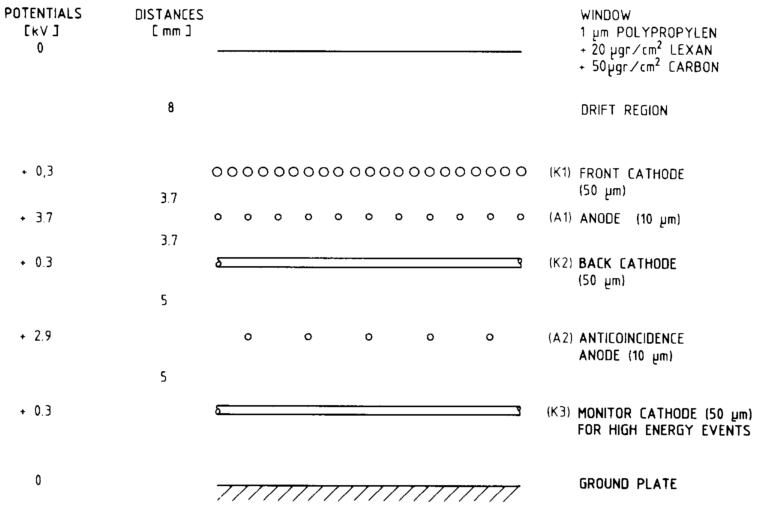
\includegraphics[width=0.7\linewidth]{figures/chapter2/rosat_pspc}
    \caption{Schematic diagram of the ROSAT PSPC \cite{rosat_pspc}. An X-ray photon enters the window and produces a photoelectron by interacting with the gas in the drift region. The photoelectron produces primary ionization electrons that drift to the front cathode and diffuse, creating a large charge cloud that involves multiple strips. These charges are accelerated by the strong electric field between the front cathode and the anode and generate ions that are collected by the front and the back cathode, giving information on the $x$ and $y$ positions. The electrodes after the back cathode are used for anticoincidence logic to reject cosmic rays.}
    \label{fig:pspc}
\end{figure}

Across the years these technologies has not evolved much in X-ray astrophysics and its use has gradually  decreased, in favor of other choices like semiconductors. In recent missions, gas detectors were mainly chosen for to cover large detection area for cost and technical reasons. \fix{devo parlare di qualcosa inerente a IXPE qui oppure rinviamo tutto a capitolo 3?}

 




















\subsection{Solid state detectors}

\fix{qui descriviamo il funzionamento di un detector a semiconduttore, con le varie proprietà, e descriviamo anche il funzionamento delle giunzioni, in particolare pn e schottky. parliamo anche della diffusione della carica all'interno del sensore.}
\fix{The interaction must occur inside the depletion region, but if we are with a fully depleted sensor we don't mind about this detail, because it is always the case}

















